\begin{figure}[htbp]
\centering
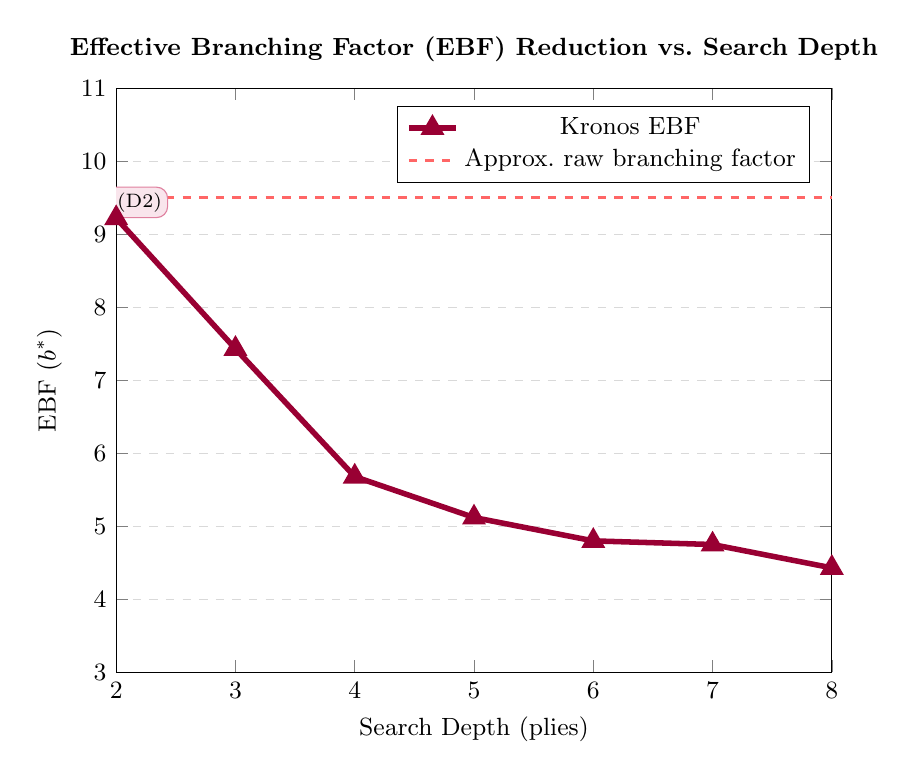
\begin{tikzpicture}
\begin{axis}[
    title style={font=\bfseries\small},
    title={Effective Branching Factor (EBF) Reduction vs.\ Search Depth},
    xlabel={Search Depth (plies)},
    ylabel={EBF ($b^*$)},
    xmin=2, xmax=8,
    ymin=3, ymax=11,
    xtick={2,3,4,5,6,7,8},
    ymajorgrids=true,
    grid style={dashed, gray!30},
    width=0.88\textwidth,
    height=9cm,
    tick label style={font=\small},
    label style={font=\small},
    legend style={font=\small, at={(0.97,0.97)}, anchor=north east}
]
\addplot[
    color=purple!80!black,
    mark=triangle*,
    mark size=3pt,
    line width=2pt
]
coordinates {
    (2, 9.22)
    (3, 7.43)
    (4, 5.68)
    (5, 5.12)
    (6, 4.80)
    (7, 4.75)
    (8, 4.43)
};

\addlegendentry{Kronos EBF}

% Reference line for approximate raw branching factor
\addplot[
    dashed,
    color=red!60,
    line width=1.2pt
]
coordinates {
    (2, 9.5)
    (8, 9.5)
};
\addlegendentry{Approx.\ raw branching factor}

% Stabilization annotation
\node[font=\scriptsize, fill=purple!10, draw=purple!50, rounded corners, inner sep=2pt,
      anchor=west] at (axis cs:8,4.43) {\textbf{4.43} (D8)};

% Start annotation
\node[font=\scriptsize, fill=purple!10, draw=purple!50, rounded corners, inner sep=2pt,
      anchor=south] at (axis cs:2,9.22) {9.22 (D2)};

\end{axis}
\end{tikzpicture}
\caption[Effective Branching Factor across Search Depths]{Effective Branching Factor (EBF) across search depths. EBF measures the geometric mean number of nodes expanded per ply. The reference line shows the approximate raw branching factor without heuristics.}

\label{fig:effective_branching_factor}
\end{figure}
% Source Material: DISCUSSION.md and search scripts
